\ifdefined\ishandout
  \documentclass[handout,landscape]{beamer} 
\else
  \documentclass[landscape]{beamer}
\fi

%\hypersetup{pdfpagemode=FullScreen} %Enabling this option will cause the slides to go full-screen on opening

\mode<handout>
{
  \usepackage{pgf}
  \usepackage{pgfpages}

\pgfpagesdeclarelayout{6 on 1 boxed}
{
  \edef\pgfpageoptionheight{\the\paperheight} 
  \edef\pgfpageoptionwidth{\the\paperwidth}
  \edef\pgfpageoptionborder{0pt}
}
{
  \pgfpagesphysicalpageoptions
  {%
    logical pages=6,%
    physical height=\pgfpageoptionheight,%
    physical width=\pgfpageoptionwidth%
  }
  \pgfpageslogicalpageoptions{1}
  {%
    border code=\pgfsetlinewidth{1pt}\pgfstroke,%
    border shrink=\pgfpageoptionborder,%
    resized width=.5\pgfphysicalwidth,%
    resized height=.5\pgfphysicalheight,%
    center=\pgfpoint{.25\pgfphysicalwidth}{.833\pgfphysicalheight}%
  }%
  \pgfpageslogicalpageoptions{2}
  {%
    border code=\pgfsetlinewidth{1pt}\pgfstroke,%
    border shrink=\pgfpageoptionborder,%
    resized width=.5\pgfphysicalwidth,%
    resized height=.5\pgfphysicalheight,%
    center=\pgfpoint{.75\pgfphysicalwidth}{.833\pgfphysicalheight}%
  }%
  \pgfpageslogicalpageoptions{3}
  {%
    border code=\pgfsetlinewidth{1pt}\pgfstroke,%
    border shrink=\pgfpageoptionborder,%
    resized width=.5\pgfphysicalwidth,%
    resized height=.5\pgfphysicalheight,%
    center=\pgfpoint{.25\pgfphysicalwidth}{.5\pgfphysicalheight}%
  }%
  \pgfpageslogicalpageoptions{4}
  {%
    border code=\pgfsetlinewidth{1pt}\pgfstroke,%
    border shrink=\pgfpageoptionborder,%
    resized width=.5\pgfphysicalwidth,%
    resized height=.5\pgfphysicalheight,%
    center=\pgfpoint{.75\pgfphysicalwidth}{.5\pgfphysicalheight}%
  }%
  \pgfpageslogicalpageoptions{5}
  {%
    border code=\pgfsetlinewidth{1pt}\pgfstroke,%
    border shrink=\pgfpageoptionborder,%
    resized width=.5\pgfphysicalwidth,%
    resized height=.5\pgfphysicalheight,%
    center=\pgfpoint{.25\pgfphysicalwidth}{.167\pgfphysicalheight}%
  }%
  \pgfpageslogicalpageoptions{6}
  {%
    border code=\pgfsetlinewidth{1pt}\pgfstroke,%
    border shrink=\pgfpageoptionborder,%
    resized width=.5\pgfphysicalwidth,%
    resized height=.5\pgfphysicalheight,%
    center=\pgfpoint{.75\pgfphysicalwidth}{.167\pgfphysicalheight}%
  }%
}


  \pgfpagesuselayout{6 on 1 boxed}[letterpaper, border shrink=5mm]
  \nofiles
}

\usepackage{listings}
\usepackage{multimedia}
\usepackage[normalem]{ulem}
\usepackage{ifthen}
\usepackage{textcomp}

\usetheme{Warsaw} 
\usecolortheme{seahorse}
\useoutertheme{infolines} 

\setbeamertemplate{blocks}[rounded][shadow=true] 

\author{Joe Fields}
\title{Introduction to Proof} 

\date{Lecture 33 (GIAM \S 6.5) \newline functions}
\institute[SCSU]{ {\tt fieldsj1@southernct.edu} }


\newlength{\cwidth}
\newcommand{\cents}{\settowidth{\cwidth}{c}%
\divide\cwidth by2
\advance\cwidth by-.1pt
c\kern-\cwidth
\vrule width .1pt depth.2ex height1.2ex
\kern\cwidth}

\newcommand{\sageprompt}{ {\tt sage$>$} }
\newcommand{\tab}{\rule{20pt}{0pt}}
\newcommand{\blnk}{\rule{1.5pt}{0pt}\rule{.4pt}{1.2pt}\rule{9pt}{.4pt}\rule{.4pt}{1.2pt}\rule{1.5pt}{0pt}}
\newcommand{\suchthat}{\; \rule[-3pt]{.25pt}{13pt} \;}
\newcommand{\divides}{\!\mid\!}
\newcommand{\tdiv}{\; \mbox{div} \;}
\newcommand{\restrict}[2]{#1 \,\rule[-4pt]{.125pt}{14pt}_{\,#2}}
\newcommand{\lcm}[2]{\mbox{lcm} (#1, #2)}
\renewcommand{\gcd}[2]{\mbox{gcd} (#1, #2)}
\newcommand{\Naturals}{{\mathbb N}}
\newcommand{\Integers}{{\mathbb Z}}
\newcommand{\Znoneg}{{\mathbb Z}^{\mbox{\tiny noneg}}}
\newcommand{\Enoneg}{{\mathbb E}^{\mbox{\tiny noneg}}}
\newcommand{\Qnoneg}{{\mathbb Q}^{\mbox{\tiny noneg}}}
\newcommand{\Rnoneg}{{\mathbb R}^{\mbox{\tiny noneg}}}
\newcommand{\Rationals}{{\mathbb Q}}
\newcommand{\Reals}{{\mathbb R}}
\newcommand{\Complexes}{{\mathbb C}}
%\newcommand{\F2}{{\mathbb F}_{2}}
\newcommand{\relQ}{\mbox{\textsf Q}}
\newcommand{\relR}{\mbox{\textsf R}}
\newcommand{\nrelR}{\mbox{\raisebox{1pt}{$\not$}\rule{1pt}{0pt}{\textsf R}}}
\newcommand{\relS}{\mbox{\textsf S}}
\newcommand{\relA}{\mbox{\textsf A}}
\newcommand{\Dom}[1]{\mbox{Dom}(#1)}
\newcommand{\Cod}[1]{\mbox{Cod}(#1)}
\newcommand{\Rng}[1]{\mbox{Rng}(#1)}

\DeclareMathOperator\caret{\raisebox{1ex}{$\scriptstyle\wedge$}}

\newtheorem*{defi}{Definition}
\newtheorem*{exer}{Exercise}
\newtheorem{thm}{Theorem}[section]
\newtheorem*{thm*}{Theorem}
\newtheorem{lem}[thm]{Lemma}
\newtheorem{cor}{Corollary}
\newtheorem{conj}{Conjecture}

\renewenvironment{proof}%
{\begin{quote} \emph{Proof:} }%
{\rule{0pt}{0pt} \newline \rule{0pt}{15pt} \hfill Q.E.D. \end{quote}}


\newcommand{\vs}{\rule{0pt}{11pt}}
\newcommand{\notimplies}{\;\not\!\!\!\implies}
\newcommand{\dx}{\,\mbox{d}x}

\AtBeginSection[]
{
 \begin{frame}{Table of Contents} 
  \tableofcontents[currentsection]
 \end{frame}
}

%%%% SAVE %%%%
%{ %magic to get a full screen image...
%\setbeamertemplate{navigation symbols}{}  % hide navigation buttons 
%\setbeamertemplate{background canvas}{\centerline{\includegraphics 
%	[height=\paperheight]{Cantor_4.jpeg}}}
%\begin{frame}[plain]
%\rule{0pt}{0pt}
%\end{frame} 
%} %end of magic


\begin{document}

\begin{frame}[plain]
  \titlepage
\end{frame}

\section{the definition}

\begin{frame}{what is a function?}
\begin{itemize}
\item We're going to be playing around, trying to find the ``right'' definition of what a function is. \pause
\item An out-dated definition:\pause \newline
\begin{defi}
 A \emph{function} $f$ is a well-defined rule, that, given any input
value $x$ produces a unique output value $f(x)$.
\end{defi}
\pause
\item That $y=f(x)$ notation (having been invented by L. Euler) is known as {\em Euler notation}. \pause
\item A more modern (but flawed) definition:\pause
\begin{defi}
 A \emph{function} is a binary relation which does not contain
distinct pairs having the same initial element.
\end{defi}
\end{itemize}
\end{frame}

\begin{frame}{Four (uhmm Three?) sets}
\begin{itemize}
\item Remember, in general a relation is some subset of $A \times B$. \pause
\item Example: $A = \{1, 2, 3, 4\}$ and $B = \{do, re, mi, fa \}$.  \pause
\item So $A\times B$ contains 16 ordered pairs. \pause
\item Suppose $\relR = \{ (1,do), (2, re), (3, mi) \}$. \pause
\item We've got 4 sets in this example: \pause
\begin{itemize}
  \item $A$, the set where the left-hand elements in the pairs in $\relR$ could potentially lie. \pause
  \item $B$, the set where the right-hand elements in the pairs in $\relR$ could potentially lie.\pause
  \item $A' = \{1, 2, 3\}$, the set of left-hand elements that actually occur in the pairs in $\relR$. \pause
  \item $B' = \{do, re, mi\}$, the set of right-hand elements that actually occur in the pairs in $\relR$. \pause
\end{itemize}
\item Perhaps a picture is in order.
\end{itemize}
\end{frame}

\begin{frame}{a picture}
\begin{picture}(0,0)%
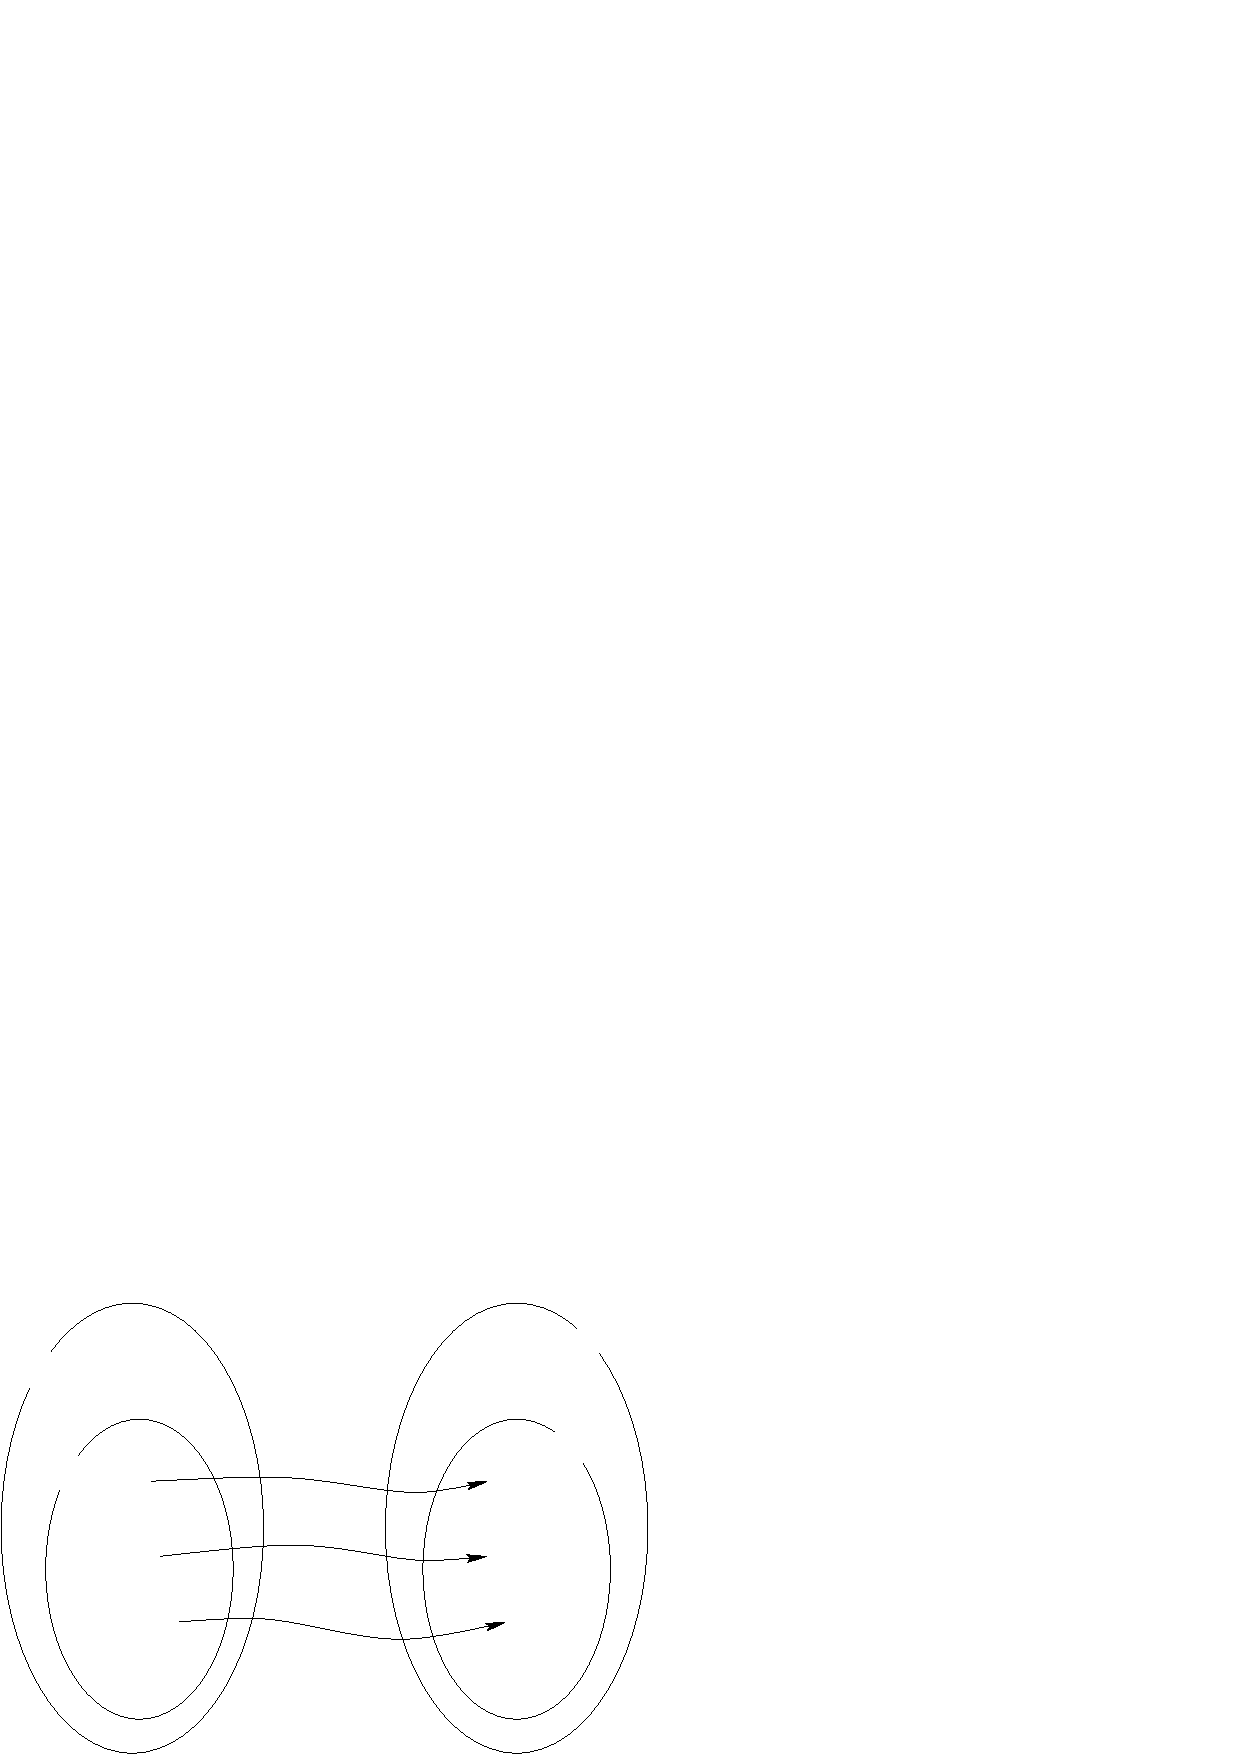
\includegraphics{./generic_function.pdf}%
\end{picture}%
\setlength{\unitlength}{3947sp}%
%
\begingroup\makeatletter\ifx\SetFigFont\undefined%
\gdef\SetFigFont#1#2#3#4#5{%
  \reset@font\fontsize{#1}{#2pt}%
  \fontfamily{#3}\fontseries{#4}\fontshape{#5}%
  \selectfont}%
\fi\endgroup%
\begin{picture}(5191,3614)(2018,-5693)
\put(2851,-2386){\makebox(0,0)[lb]{\smash{{\SetFigFont{12}{14.4}{\rmdefault}{\mddefault}{\updefault}{\color[rgb]{0,0,0}$a$}%
}}}}
\put(3151,-2761){\makebox(0,0)[lb]{\smash{{\SetFigFont{12}{14.4}{\rmdefault}{\mddefault}{\updefault}{\color[rgb]{0,0,0}$b$}%
}}}}
\put(3001,-3586){\makebox(0,0)[lb]{\smash{{\SetFigFont{12}{14.4}{\rmdefault}{\mddefault}{\updefault}{\color[rgb]{0,0,0}$c$}%
}}}}
\put(3076,-4186){\makebox(0,0)[lb]{\smash{{\SetFigFont{12}{14.4}{\rmdefault}{\mddefault}{\updefault}{\color[rgb]{0,0,0}$d$}%
}}}}
\put(3226,-4711){\makebox(0,0)[lb]{\smash{{\SetFigFont{12}{14.4}{\rmdefault}{\mddefault}{\updefault}{\color[rgb]{0,0,0}$e$}%
}}}}
\put(6001,-2461){\makebox(0,0)[lb]{\smash{{\SetFigFont{12}{14.4}{\rmdefault}{\mddefault}{\updefault}{\color[rgb]{0,0,0}$v$}%
}}}}
\put(6001,-2761){\makebox(0,0)[lb]{\smash{{\SetFigFont{12}{14.4}{\rmdefault}{\mddefault}{\updefault}{\color[rgb]{0,0,0}$w$}%
}}}}
\put(6001,-3511){\makebox(0,0)[lb]{\smash{{\SetFigFont{12}{14.4}{\rmdefault}{\mddefault}{\updefault}{\color[rgb]{0,0,0}$x=f(c)$}%
}}}}
\put(6001,-4111){\makebox(0,0)[lb]{\smash{{\SetFigFont{12}{14.4}{\rmdefault}{\mddefault}{\updefault}{\color[rgb]{0,0,0}$y=f(d)$}%
}}}}
\put(6151,-4636){\makebox(0,0)[lb]{\smash{{\SetFigFont{12}{14.4}{\rmdefault}{\mddefault}{\updefault}{\color[rgb]{0,0,0}$z=f(e)$}%
}}}}
\put(2476,-3511){\makebox(0,0)[lb]{\smash{{\SetFigFont{12}{14.4}{\rmdefault}{\mddefault}{\updefault}{\color[rgb]{0,0,0}$A'$}%
}}}}
\put(2251,-2686){\makebox(0,0)[lb]{\smash{{\SetFigFont{12}{14.4}{\rmdefault}{\mddefault}{\updefault}{\color[rgb]{0,0,0}$A$}%
}}}}
\put(6676,-2461){\makebox(0,0)[lb]{\smash{{\SetFigFont{12}{14.4}{\rmdefault}{\mddefault}{\updefault}{\color[rgb]{0,0,0}$B$}%
}}}}
\put(6526,-3286){\makebox(0,0)[lb]{\smash{{\SetFigFont{12}{14.4}{\rmdefault}{\mddefault}{\updefault}{\color[rgb]{0,0,0}$B'$}%
}}}}
\end{picture}%

\end{frame}

\begin{frame}{domains}
\begin{itemize}
\item The mathematics community seems to have collectively decided to ignore the distinction between $A$ and $A'$. \pause
\item (for functions) \pause
\item When $f$ is a function, we insist that it have a value for every input in the set $A$.\pause
\item In other words, we insist that $A = \Dom{f}$.\pause
\item Oddly, we're ok with there being a superset/subset relationship on the output side.
\end{itemize}
\end{frame}


\begin{frame}{Three sets}
\begin{itemize}
\item The {\em domain} of $f$, $\Dom{f}$:\pause \newline
the set of left-hand elements that actually occur in the pairs in $f$. \pause
\item The {\em range} of $f$, $\Rng{f}$: \pause \newline
the set of right-hand elements that actually occur in the pairs in $f$. \pause
\item The {\em codomain} of $f$, $\Cod{f}$: \pause \newline
a superset of $\Rng{f}$.
\end{itemize}
\end{frame}

\begin{frame}{finally$\ldots$}
\begin{itemize}
\item The official definition of a function involves two elements:\pause
\begin{itemize}
  \item A function must be {\em defined} on its domain. \pause
  \item A rule that encapsulates the vertical line test. \pause
\end{itemize}
\item So, finally, here's the definition: \pause

\begin{defi}
If $A$ and $B$ are sets, then $f$ is a function from $A$ to $B$ (which
is expressed symbolically by $f:A\longrightarrow B$), if and only if
$f$ is a relation from $A$ to $B$, $\Dom{f}=A$ and $((a,b) \in f \; \land \; (a,c) \in f) \; \implies \; b=c$.
\end{defi}
\item We should re-interpret that using the Euler notation for functions.\pause
\item The vertical line test.
\end{itemize}
\end{frame}

\section{properties}

\begin{frame}{onto}
\begin{itemize}
\item ``Onto'' means that everything in the codomain is actually in the range.\pause
\item I.e. every $y$ in $\Cod{f}$ has an $x$ in $\Dom{f}$ such that $y=f(x)$.
\item It's marginally cooler to say that $f$ is a {\em surjection}. \pause
\item Alternatively: $f$ is {\em surjective}. \pause
\item 
\[ f \; \mbox{is surjective} \; \iff \; \forall y \in \Cod{f}, \, \exists x \in \Dom{f}, \, f(x) = y \]
\end{itemize}
\end{frame}

\begin{frame}{one-to-one}
\begin{itemize}
\item ``One-to-one'' probably should be thought of as {\em not} many-to-one. \pause
\item For instance, $f(x) = x^2$ is (usually) two-to-one. \pause \newline
(Except when $x=0$, $x$ and $-x$ are distinct, and both get sent to the same number.)\pause
\item That means $f(x)$ is {\em not} one-to-one. \pause
\item But, for example $g(x) = e^x$ is one-to-one.
\item The fancier terminology is: ``$g$ is an {\em injection}'' or ``$g$ is {\em injective}.'' \pause
\item 
\[ f \; \mbox{is injective} \; \iff \; \forall x_1, x_2 \in \Dom{f}, \, (f(x_1) = f(x_2))\, \implies \, x_1 = x_2 \]
\end{itemize}
\end{frame}

\begin{frame}{restricting domains}
\begin{itemize}
\item Since being injective is a desireable property, and many functions aren't, there is a standard trick for getting an injective function from some other function.\pause
\item Restricting the domain.\pause
\item Basically, just declare that one of the $x$'s that gets mapped to a particular $y$ is the winner, and remove any other inputs that go to that $y$ from the domain. \pause
\item $f(x) = x^2; x \geq 0$ \pause
\item Desmos
\item The horizontal line test.
\end{itemize}
\end{frame}

\begin{frame}{the inverse}
\begin{itemize}
\item As we've seen, every relation $\relR$ has an inverse, $\relR^{-1}$ defined by
\[ \relR^{-1} \; = \; \{ (y,x) \, \suchthat \, (x,y) \in \relR \} \]
\pause
\item Often, people will say that a certain function doesn't have an inverse, but that's not true! \pause
\item Every function is a relation, and since every function is a relation, they all have inverses! \pause
\item What people really mean is that the inverse is not itself a function. \pause
\item Being injective is precisely what's needed to guarantee that your inverse will be a function.
\end{itemize}
\end{frame}

\section{bijections}

\begin{frame}{images and preimages}
\begin{itemize}
\item Bijections are functions that are both surjective and injective. \pause
\item Before going any further with that we'll introduce some terminology that makes it easier to talk about these things:\ pause
\item When $y = f(x)$ we say that ``$y$ is the image of $x$.'' \pause
\item If there are several functions floating around you can be more explicit by saying \newline
``$y$ is the image of $x$ under $f$.'' \pause
\item In a similar vein we can say that ``$x$ is a preimage of $y$'' or  ``$x$ is a preimage of $y$ under $f$'' 
\item Articles: ``the'' vs. ``a'' \pause (definite vs. indefinite article) \pause
\item When a function is injective, preimages become unique, so (assuming $f$ is one-to-one) it's okay to say ``the preimage of $y$.''
\end{itemize}
\end{frame}

\begin{frame}{definition of a bijection}
\begin{itemize}
\item A function $f$ that is both injective and surjective is a {\em bijection}. \pause
\item ``Surjective'' means every $y \in \Cod{f}$ has a preimage in $\Dom{f}$. \pause
\item ``Injective'' means that that preimage is unique. \pause
\end{itemize}
\end{frame}

\begin{frame}{proving that a function is a bijection}
\begin{itemize}
\item Example on page 282.
\item A more complicated example starts on page 283.
\end{itemize}
\end{frame}


\begin{frame}{images and preimages of sets}
\begin{itemize}
\item We can extend the ideas of images and preimages to sets. \pause
\item When $A \subseteq \Dom{f}$, {\em the image of $A$} is defined as 
\[ f(A) \; = \; \{ f(a) \, \suchthat \, a \in A \}. \]
\pause
\item Preimages of sets are denoted $f^{-1}(B)$ -- the image of $B$ under the inverse function for $f$. \pause \newline
(Even though there might not be an inverse function!) \pause
\item When $B \subseteq \Cod{f}$, {\em the preimage of $B$} is defined as 
\[ f^{-1}(B) \; = \; \{ x \, \suchthat \, f(x) \in B \}. \]
\pause
\end{itemize}
\end{frame}

\begin{frame}{Once more into the breach}
\begin{itemize}
\item Let's talk about one-to-one and onto in terms of this new ``sets'' version of image and preimage. \pause
\item Surjective: \pause \newline
$f:A \longrightarrow B$ is {\em onto} provided that $f(A) = B$. \pause
\item Injective: \pause \newline
$f:A \longrightarrow B$ is {\em one-to-one} provided that all inverse images of singleton sets are singleton sets.
\end{itemize}
\end{frame}


\end{document}
